%
% Optimising the World
%

\section{Optimising the world}\label{sec:optimising_the_world}\index{Optimisation}

Every aspect of our modern world is heavily optimised to improve efficiency, affordability, profitability, and every other kind of desirability. Even long before the digital revolution, which enabled the widespread implementation of modern optimisation-theoretic techniques, humans have always striven to make life as easy as possible -- the least effort for the greatest possible reward. Our modern application of optimisation theory is merely a logical extension of this to the many other facets of the 21st century economy that now exist.

\subsection{Optimisation in everyday life}

Broadly speaking, optimisation problems can all in some sense be thought of as \textit{resource allocation} problems\index{Resource allocation} -- given finite resources, that we would like to utilise most efficiently and for the greatest reward, what is the best way to allocate and distribute them within a complex system?

To lay the context for the remainder of the section, and illustrate the importance and transformative potential for improved optimisation approaches, we summarise several familiar everyday applications for optimisation theory that we all rely on, usually unwittingly, executed somewhere in the background up in the cloud, the end user oblivious to the gargantuan calculations being performed behind the scenes merely to update a barely noticeable on-screen logo. There are countless more examples than we can't possibly have the time and space to comprehensively summarise here.

The examples we present are all examples of \textit{satisfiability problems}\index{Satisfiability problems} -- the problem of trying to simultaneously satisfy a large number of potentially competing constraints in a system, with the best possible outcome.

It is well known that the most complex such satisfiability problems are \textbf{NP}-complete\index{\textbf{NP}-complete} in general, with no known efficient classical solutions (in fact even very trivial constructions of satisfiability problems are already \textbf{NP}-complete, e.g see Fig.~\ref{fig:3SAT}).

Here are a mere few notable everyday applications for optimisation theory.

\subsubsection{Traffic networks}\index{Traffic networks}

Given our highly interconnected road networks, what is the best route to take to get home, given the  complex and often unpredictable dynamics of road traffic? And how does that answer change when potentially millions of travellers are simultaneously competing to minimise their individual travel times?

To implement a straightforward {\sc Greedy} strategy, a simple application of Dijkstra's shortest path algorithm (Sec.~\ref{sec:shortest_path}) will yield the optimal route for an individual user, and very quickly since it has only $O(n^2)$ complexity (i.e a \textbf{P} algorithm).

However, in such multi-user systems, with so many users, {\sc Greedy}\index{Greedy strategy} strategies, based on optimising users individually, are highly sub-optimal, and globally optimised algorithms must be pursued. For example, if there are a thousand drivers competing to get from Town Hall to Redfern, it makes no sense to optimise them individually, since then they will all be identically directed down George St, which will of course quickly saturate and congest. Obviously load-balancing across the various routes benefits everyone collectively \textit{and} individually.

The complexities of a global multi-user optimisation are intuitively evident -- with countless competing interests, finding a set of routes that minimises net transit time yields an enormous space of possibilities and variations to consider, far beyond individual optimisations performed independently. Alas, Dijkstra's tempting algorithm is not very useful, and we must employ harder algorithms, many of which are \textbf{NP}-complete. Some of these were introduced in the context of network packet routing algorithms in Sec.~\ref{sec:route_strats}, a conceptually identical problem to road traffic routing.

Fig.~\ref{fig:traffic_opt} provides a simple example illustrating how individual local optimisations can yield suboptimal routing, with a global optimisation yielding a better overall outcome.

\begin{figure*}[!htb]
	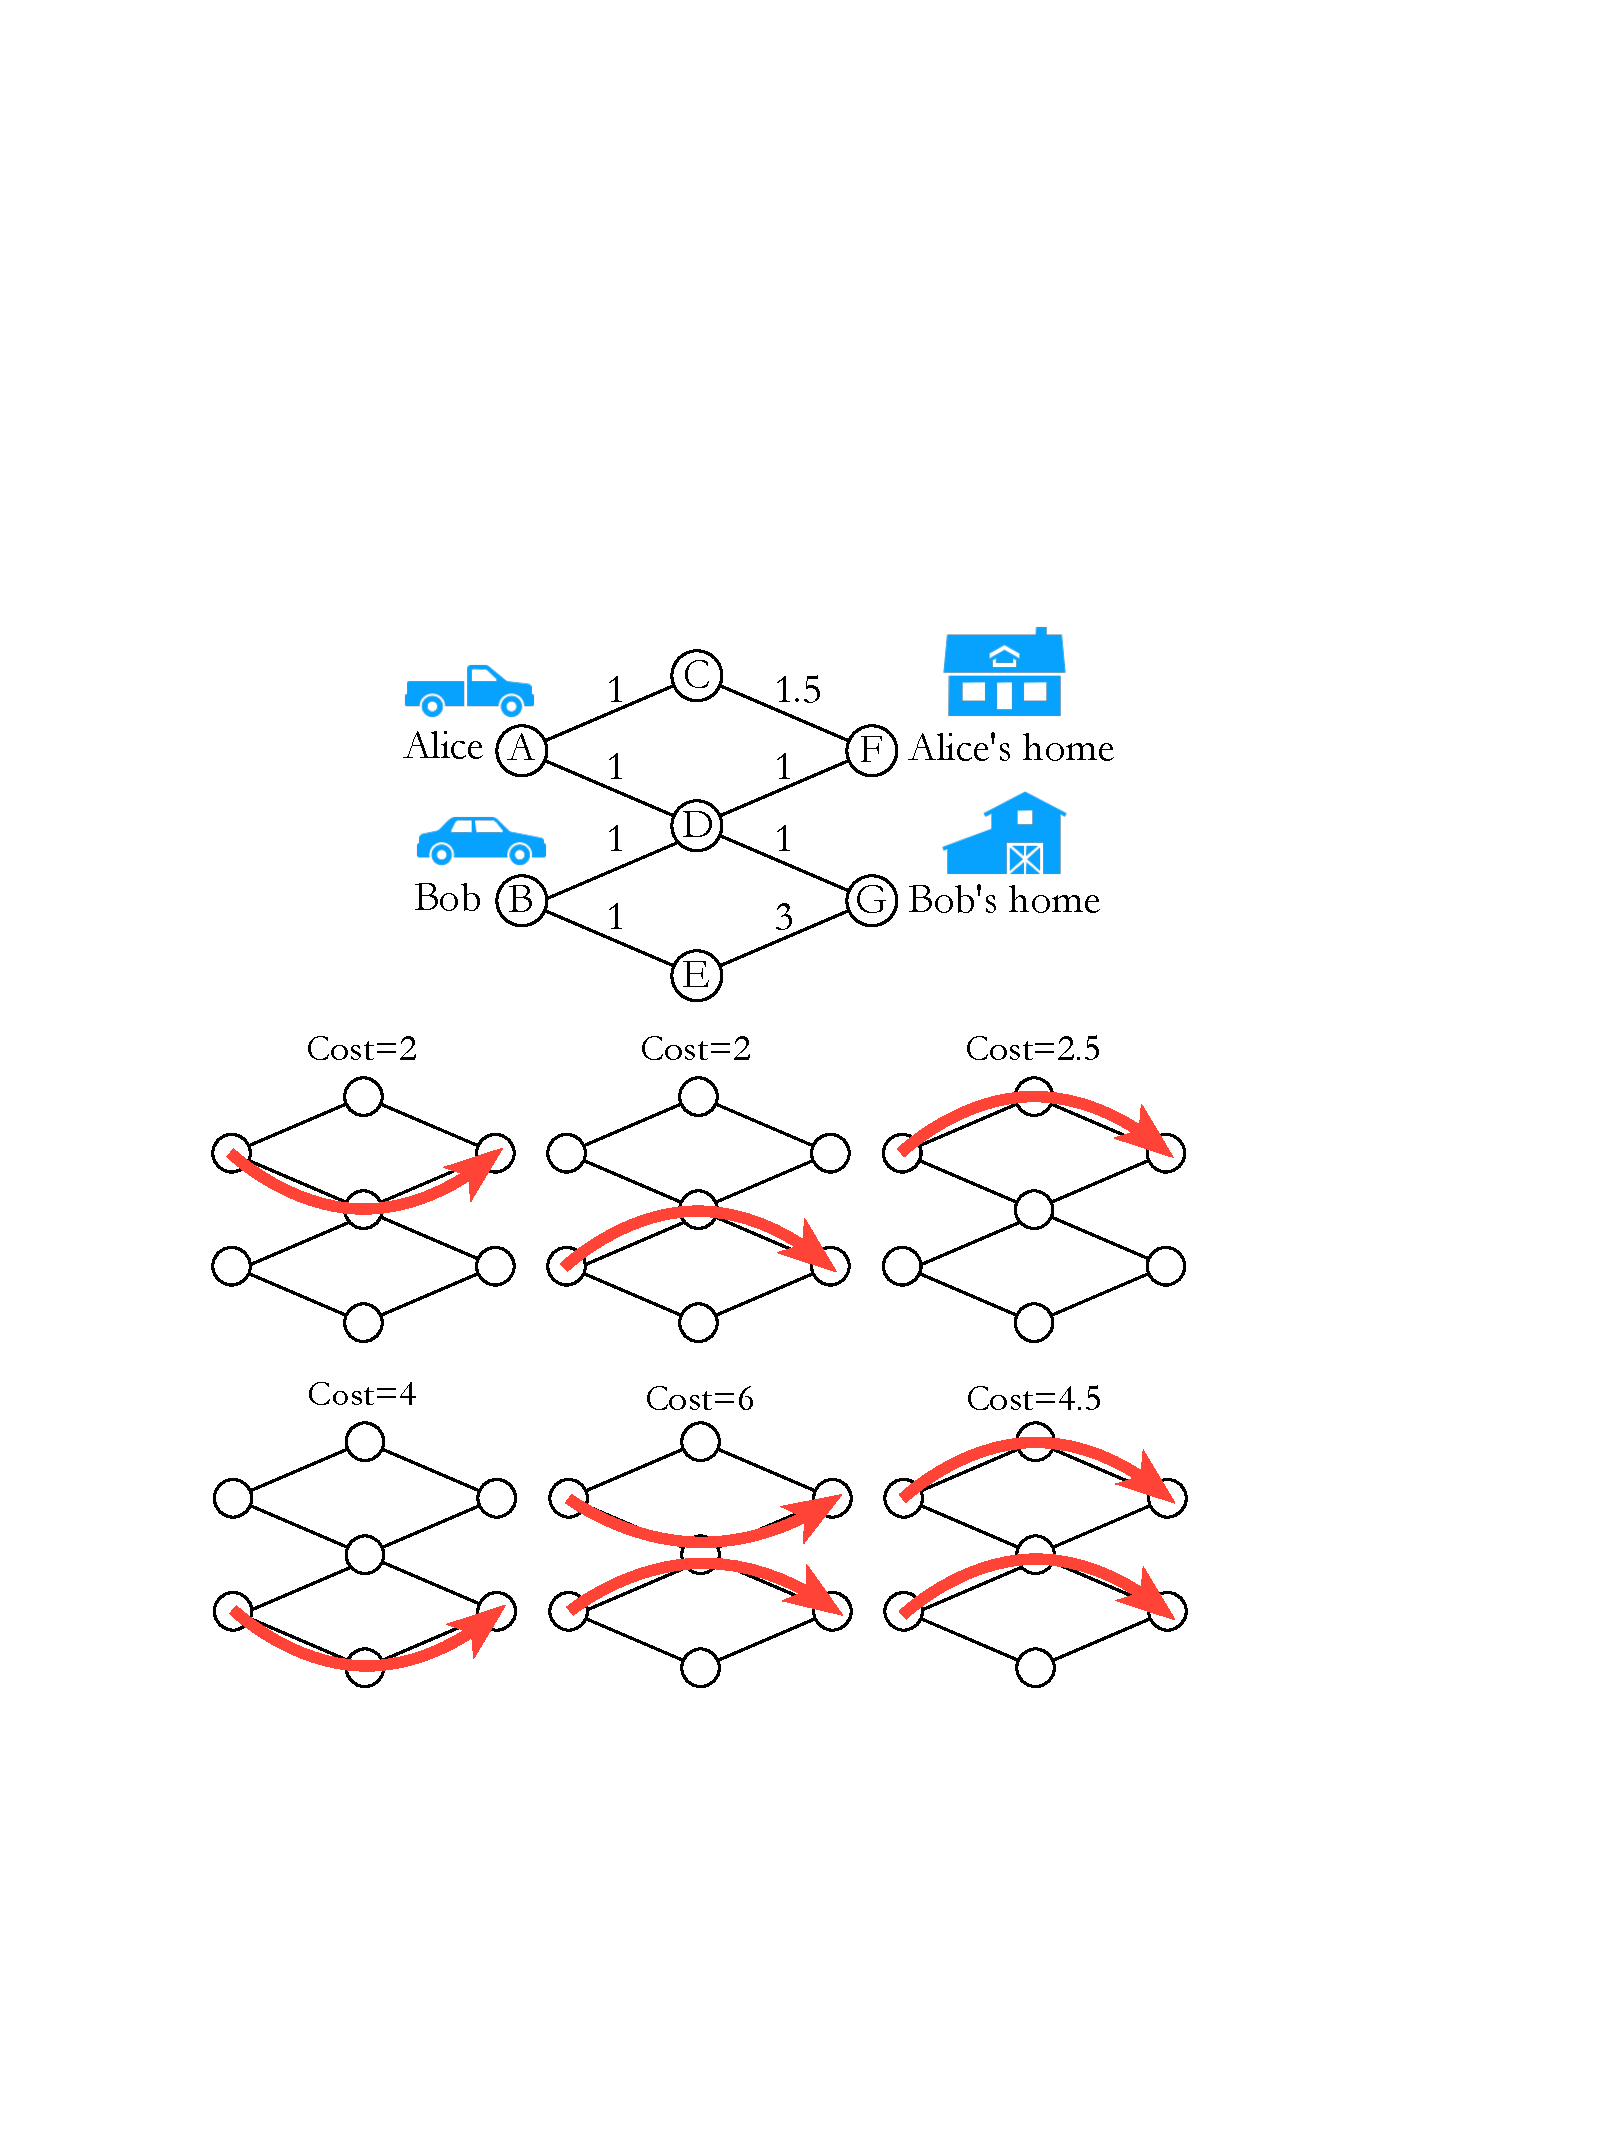
\includegraphics[width=0.6\textwidth]{traffic_optimisation}
	\caption{Simple road network, where vertices represent intersections and edges represent roads. Edge weights indicate their associated travel time. The goal is for Alice and Bob to both drive home optimally, i.e minimising net commute time. Let us assume that the intersections do not delay single cars, but if they become congested (i.e more than one car simultaneously) they induce a time delay of 1 on all drivers present at the intersection. If Bob were to stay at work, and only Alice was attempting to drive home, her optimal route would be \mbox{$A\to D\to F$}, with a commute time of 2. Conversely, if Alice stayed at work and Bob was driving home, his optimal route would be \mbox{$B\to D\to G$}, also with a commute time of 2. However, if both Alice and Bob were driving home at the same time there would be congestion at intersection $D$, and their combined travel time would be 6, not the intended 4. Thus, by optimising their routes independently of one another their competition for intersection $D$ would penalise both of them by 1. On the other hand, a global optimisation would show that a more optimal routing would be for Alice to take \mbox{$A\to C\to F$} (time 2.5), with Bob remaining on \mbox{$B\to D\to G$} (time 2). This would penalise Alice by only 0.5 for taking the longer road, but both Alice and Bob would no longer be penalised at the congested intersection, reducing their collective transit time to 4.5, a saving of 1.5. Note that Alice and Bob are not only better off collectively (i.e their joint travel time), but also individually. That is, Alice making the sacrifice of taking the longer route home actually benefits her individually, with an individual saving of 0.5. In this trivial example there is only one point of conflict in the network. In general, as the number of users scales up, the distinct ways in which combinations of conflicts could emerge grows exponentially.}\label{fig:traffic_opt}
\end{figure*}

\subsubsection{Public transport scheduling}\index{Public transport scheduling}

Given a fixed network of train lines, and a fixed number of trains, but the ability to schedule them freely, how does one schedule a roster that minimises average waiting times?

This might seem straightforward in simple test-cases. As before, optimising a single route, or several independent routes is trivial. But once complex, conflicting interdependencies are in place, conflict resolution becomes impossible to eliminate. Scheduling the Epping train to leave 5 minutes earlier will allow its passengers to catch the 5pm Hornsby train. But by leaving those few minutes earlier, passengers arriving from the Blue Mountains train will miss their connection and have to wait for the next one.

We are once again in a situation where we are overwhelmed with exponentially growing combinatorics to try and minimise the countless possible schedule conflicts that can occur. It is obvious upon inspection that finding a global optimum to this problem will not be possible via independent local optimisations, which do not accommodate for competing interdependencies. 

The importance of this problem is obvious. Minimising the resources required to operate public transport effectively could save enormous amounts of money in state budgets. Not to mention, passenger waiting time is of value too. If a million passengers lose just a few minutes of productivity per day to increased commute times, this can amount to billions of dollars a year in lost productivity to the broader economy.

\subsubsection{Economics}\index{Economics}

Governments inevitably have finite budgets\footnote{Except in Venezuela.}, and must therefore allocate tax revenue optimally. Public spending is associated with many of the same combinatorial difficulties as the previous examples.

The countless sectors of the economy are all interdependent with one another, and raise their own demands (constraints), which must be mutually satisfied. A minor misallocation of funding to one government project could have flow-on effects to other interdependent programs, yielding another resource allocation nightmare.

Of course, these ideas don't just apply to government budgets, but also budgets at smaller scales, say within a large corporation with many distinct spending programs.

\subsubsection{Supply chain networks}\index{Supply chain networks}

The modern economic infrastructure for the production and distribution of goods is built upon supply chains -- complex, interdependent networks of the exchange of resources between entities as goods pass through their many stages of production before reaching the consumer. Each exchange of resources will typically be subject to its own constraints, such as strict time of arrival demands. Effectively this yields a massive instance of a complex satisfiability problem, where all, or as many as possible of the demands of the units in the chain must be simultaneously met. Conceivably, a single unsatisfied demand may break the functionality of the entire supply chain! 

Bearing in mind that modern supply chains may be dealing with billions of dollars in resources at any given time, even minor improvements to their optimisation could be of enormous monetary value.

\subsection{Classical optimisation techniques}\index{Classical optimisation techniques}

Classical techniques for attacking optimisation problems, such as the ones presented above, typically come in the following flavours:
\begin{itemize}
	\item Heuristics\index{Heuristics}: efficient algorithms that find suboptimal, but satisfactory \textit{approximations} to the solution to a problem. These algorithms are fast and can be efficiently implemented classically, but can have highly variable accuracy in the solution they provide.
	\item Brute-force\index{Brute-force}: use raw computational power to exhaustively work through all the combinatorics of a problem. This is guaranteed to find the optimal solution, but is typically extremely slow and limited to small instances of the problem.
	\item Efficient classical algorithms: in the most ideal scenario, we may not need either of the above, since efficient classical optimisation algorithms may exist. Perhaps the best-known example of this is \textit{linear programming}\index{Linear programming}, whereby the relationships between entities in a system are defined via linear transformations. This class of problems is classically efficient to solve exactly. Clearly this won't solve \textbf{NP}-complete optimisation problems, but there are nonetheless many problems of interest in this category.
\end{itemize}

These techniques present us with a tradeoff between the optimality of a solution and the computational resources required to obtain it. Can quantum technology improve this tradeoff?

\subsection{Quantum enhancement}

We now provide a non-comprehensive overview of some of the better-known quantum optimisation algorithms. The speedups offered by these algorithms vary enormously, from simple quadratic enhancements all the way to exponential enhancement.

\subsubsection{Satisfiability problems}

%Many readers will have heard of the \textit{travelling salesman problem}\index{Travelling salesman problem}, the task of finding the shortest route through a weighted graph that traverses every vertex. This task is known to be \textbf{NP}-complete.\index{\textbf{NP}-complete}

%Many other algorithms are also known to be \textbf{NP}-complete, a number of which that are relevant to networking are discussed in detail in Sec.~\ref{sec:graph_theory}, summarised in Table.~\ref{tab:net_alg_sum}.

Alas, satisfiability and \textbf{NP}-complete problems are not believed to be efficiently solvable on quantum computers. This rules out a quantum future where the world's resources are perfectly allocated and optimised.

However, such problems can be \textit{quadratically} enhanced in runtime by cunningly employing Grover's search algorithm (Sec.~\ref{sec:quantum_search}). To see this, note that all \textbf{NP}-complete problems can be efficiently mapped to one another with polynomial resource overhead (see Fig.~\ref{fig:complexity_classes}). Thus, we can restrict ourselves to considering the satisfiability problems\index{Satisfiability problems} discussed above -- the archetypal \textbf{NP}-complete problems. An example of the 3-\textsc{SAT} problem\index{3-SAT problem}, which is \textbf{NP}-complete, is shown in Fig.~\ref{fig:3SAT}.

\begin{figure}[!htb]
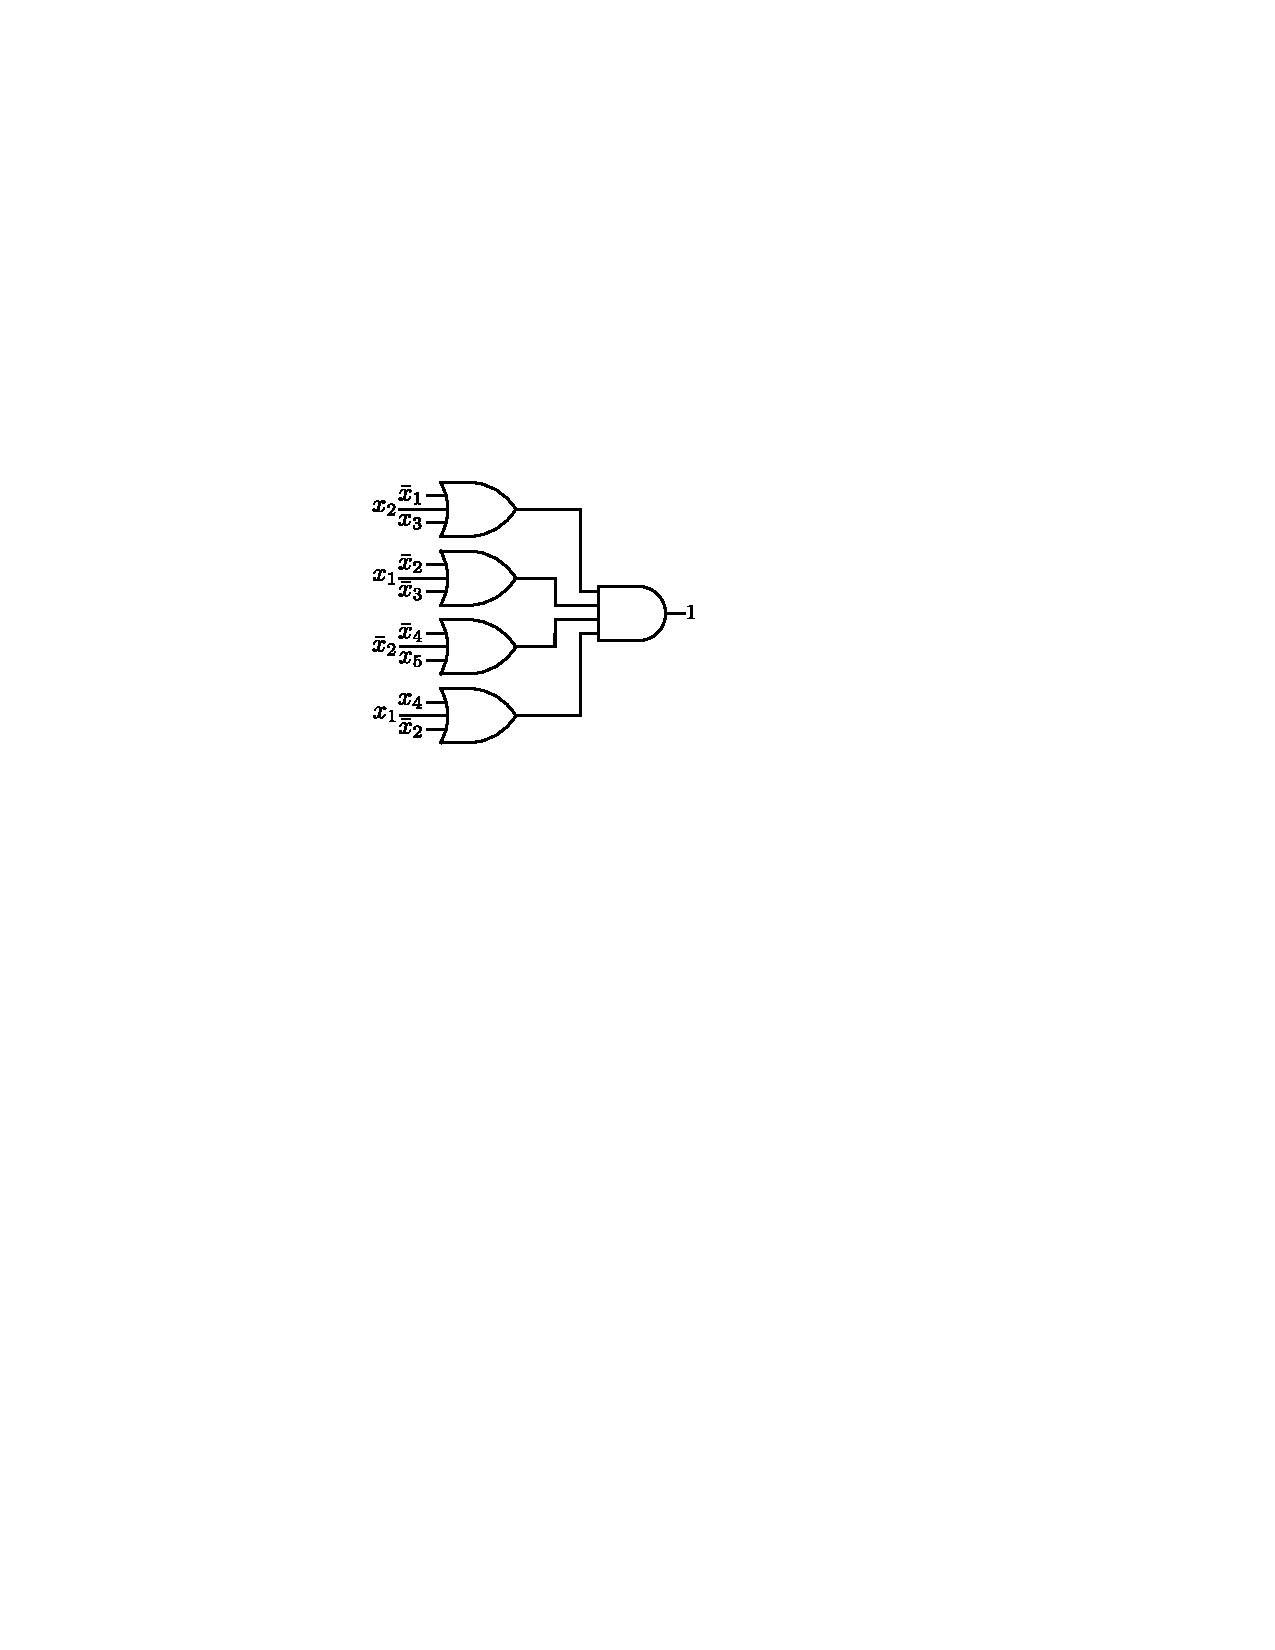
\includegraphics[width=0.3\textwidth]{3SAT}
\caption{Digital circuit for an instance of the 3-\textsc{SAT} problem, with 4 clauses acting on input variables $\{x_i\}$. Each of the OR gates is input with some combination of 3 of the input bits or their compliments (i.e with a NOT gate). Each of these is referred to as a `clause', of which there are 4 in this example, but could be any number in general. The final AND gate requires that all clauses be simultaneously satisfied in order to yield a final output of `1'. The goal of the problem is to find an input bit-string $x$ that yields an output of `1'. In general, this may require exhaustively searching over the entire space of input states via brute-force, which exhibits time-complexity exponential in the length of the bit-string and associated number of clauses. This problem is proven to be \textbf{NP}-complete. Note that the similarly-defined 2-\textsc{SAT}\index{2-SAT problem} problem (i.e clauses each contain 2 input bits) is \textbf{P}, making 3-\textsc{SAT} the simplest model to consider in the study of \textbf{NP}-complete problems. For this reason 3-\textsc{SAT} is often used as the computational model when studying \textbf{NP}-complete problems.} \label{fig:3SAT}	
\end{figure}

By defining an oracle\index{Oracle} that implements a polynomial-time algorithm on $n$ qubits, a Grover search over the input space of $O(2^n)$ configurations will determine the satisfying input to the oracle for a given desired output, which acts as the tagged element within the search algorithm. The Grover search yields a quadratic speedup for this search compared to a brute-force classical search, therefore requiring only $O(2^{n/2})$ oracle calls. While this is short of the exponential speedup one might hope for, a quadratic speedup can nonetheless be very significant for large problem instances, where even minor improvements could be of enormous value.

\subsubsection{Non-satisfiability-based optimisation algorithms}

The optimisation problems discussed until now have been satisfiability problems residing in \textbf{NP}-complete, limited to only quadratic quantum enhancement owing to their utilisation of Grover's algorithm. Are there any other optimisation problems to which quantum computers lend themselves, potentially with the cherished exponential enhancement. There are, although the examples are far less ubiquitous than the plethora of satisfiability-based optimisation problems.

\subsubsection{Least squares fitting}

A quantum-enhanced algorithm for performing least squares fitting\index{Least squares fitting} was described by \cite{HHL?}, potentially offering exponential enhancement, depending on the sparsity of the data.

As input it takes a set of data-points, \mbox{$(x_i,y_i)$}, and functions, $f_j$, outputting a set of coefficients, $\lambda_k$, defining a linear combination of those functions that fits the data, as well as a parameter characterising the quality of the fit, $E$. That is, we find the $\lambda$ that defines the fitting function\index{Fitting function},
\begin{align}
f_{\vec\lambda(x)} = \sum_k \lambda_k f_k(x),
\end{align}
such that the quality estimator\index{Quality estimator} is minimised according to a sum-of-squares\index{Sum of squares} metric,
\begin{align}
E = \sum_i |f_{\vec\lambda}(x_i)-y_i|^2.	
\end{align}

This can be thought of as an optimisation problem in the sense that our goal is to find a linear combination of functions that maximises the fit quality. This problem finds widespread use across many fields, particularly in statistics where it is ubiquitous.

\subsubsection{Semidefinite programming}

Semidefinite programming\index{Semidefinite programming} is a technique for finding solutions to constrained linear systems\index{Linear systems}. Although the technique is already classically efficient, running in polynomial time, a quantum-enhanced version has been described \cite{???}, which promises exponential speedup in certain parameter regimes.

\comment{To do}

\subsection{Approximate optimisation}\index{Approximate optimisation}

Some problems in even harder classes than \textbf{NP}-complete can in some instances be \textit{approximated} using the same approach. The key to solving such problems is to define an oracle\index{Oracle} that attributes a \textit{score}\index{Score} to a given input, rather than a yes/no answer to perfect satisfiability, and answers `yes' or `no' depending on whether that score is above some defined threshold for approximation. As an illustrative example, consider the optimisation of, say, a complex traffic network, where the goal is to maximise flow through the network. Then we might define our score to be some flow metric for the network's graph.

We then apply a Grover search repeatedly, each time incrementing this threshold until the algorithm outputs `no'. Then we know that the last input yielding the `yes' outcome had the highest score. The reason this approach is \textit{approximate} rather than \textit{exact} is that defining such a score-oracle mightn't be always efficiently implemented, or maybe it mightn't make sense at all to define score measures for a given problem. Alternately, maybe a particular problem inherently requires perfect satisfiability, and any imperfect approximation is insufficient -- if even a single constraint isn't satisfied, the system is broken.

An intuitive example of a problem taken from a far harder complexity class than \textbf{NP}-complete, that can be approximately optimised using the Grover approach is the game of chess\index{Chess}. Generalisation of the rules of chess to an \mbox{$n\times n$} board yields a game proven to reside in \textbf{EXP}-complete\index{\textbf{EXP}-complete} -- the class of all problems requiring exponential runtime on a classical computer.

How do current classical computers play chess? They construct a \textit{search tree}\index{Search tree} (see Fig.~\ref{fig:search_tree}), which is explored exhaustively up to a given depth (bounded by computational resources), and assign a score to each board position, indicating the relative strength of its position. The branch in the tree with the highest scores determines the next move.

\begin{figure}[!htb]
	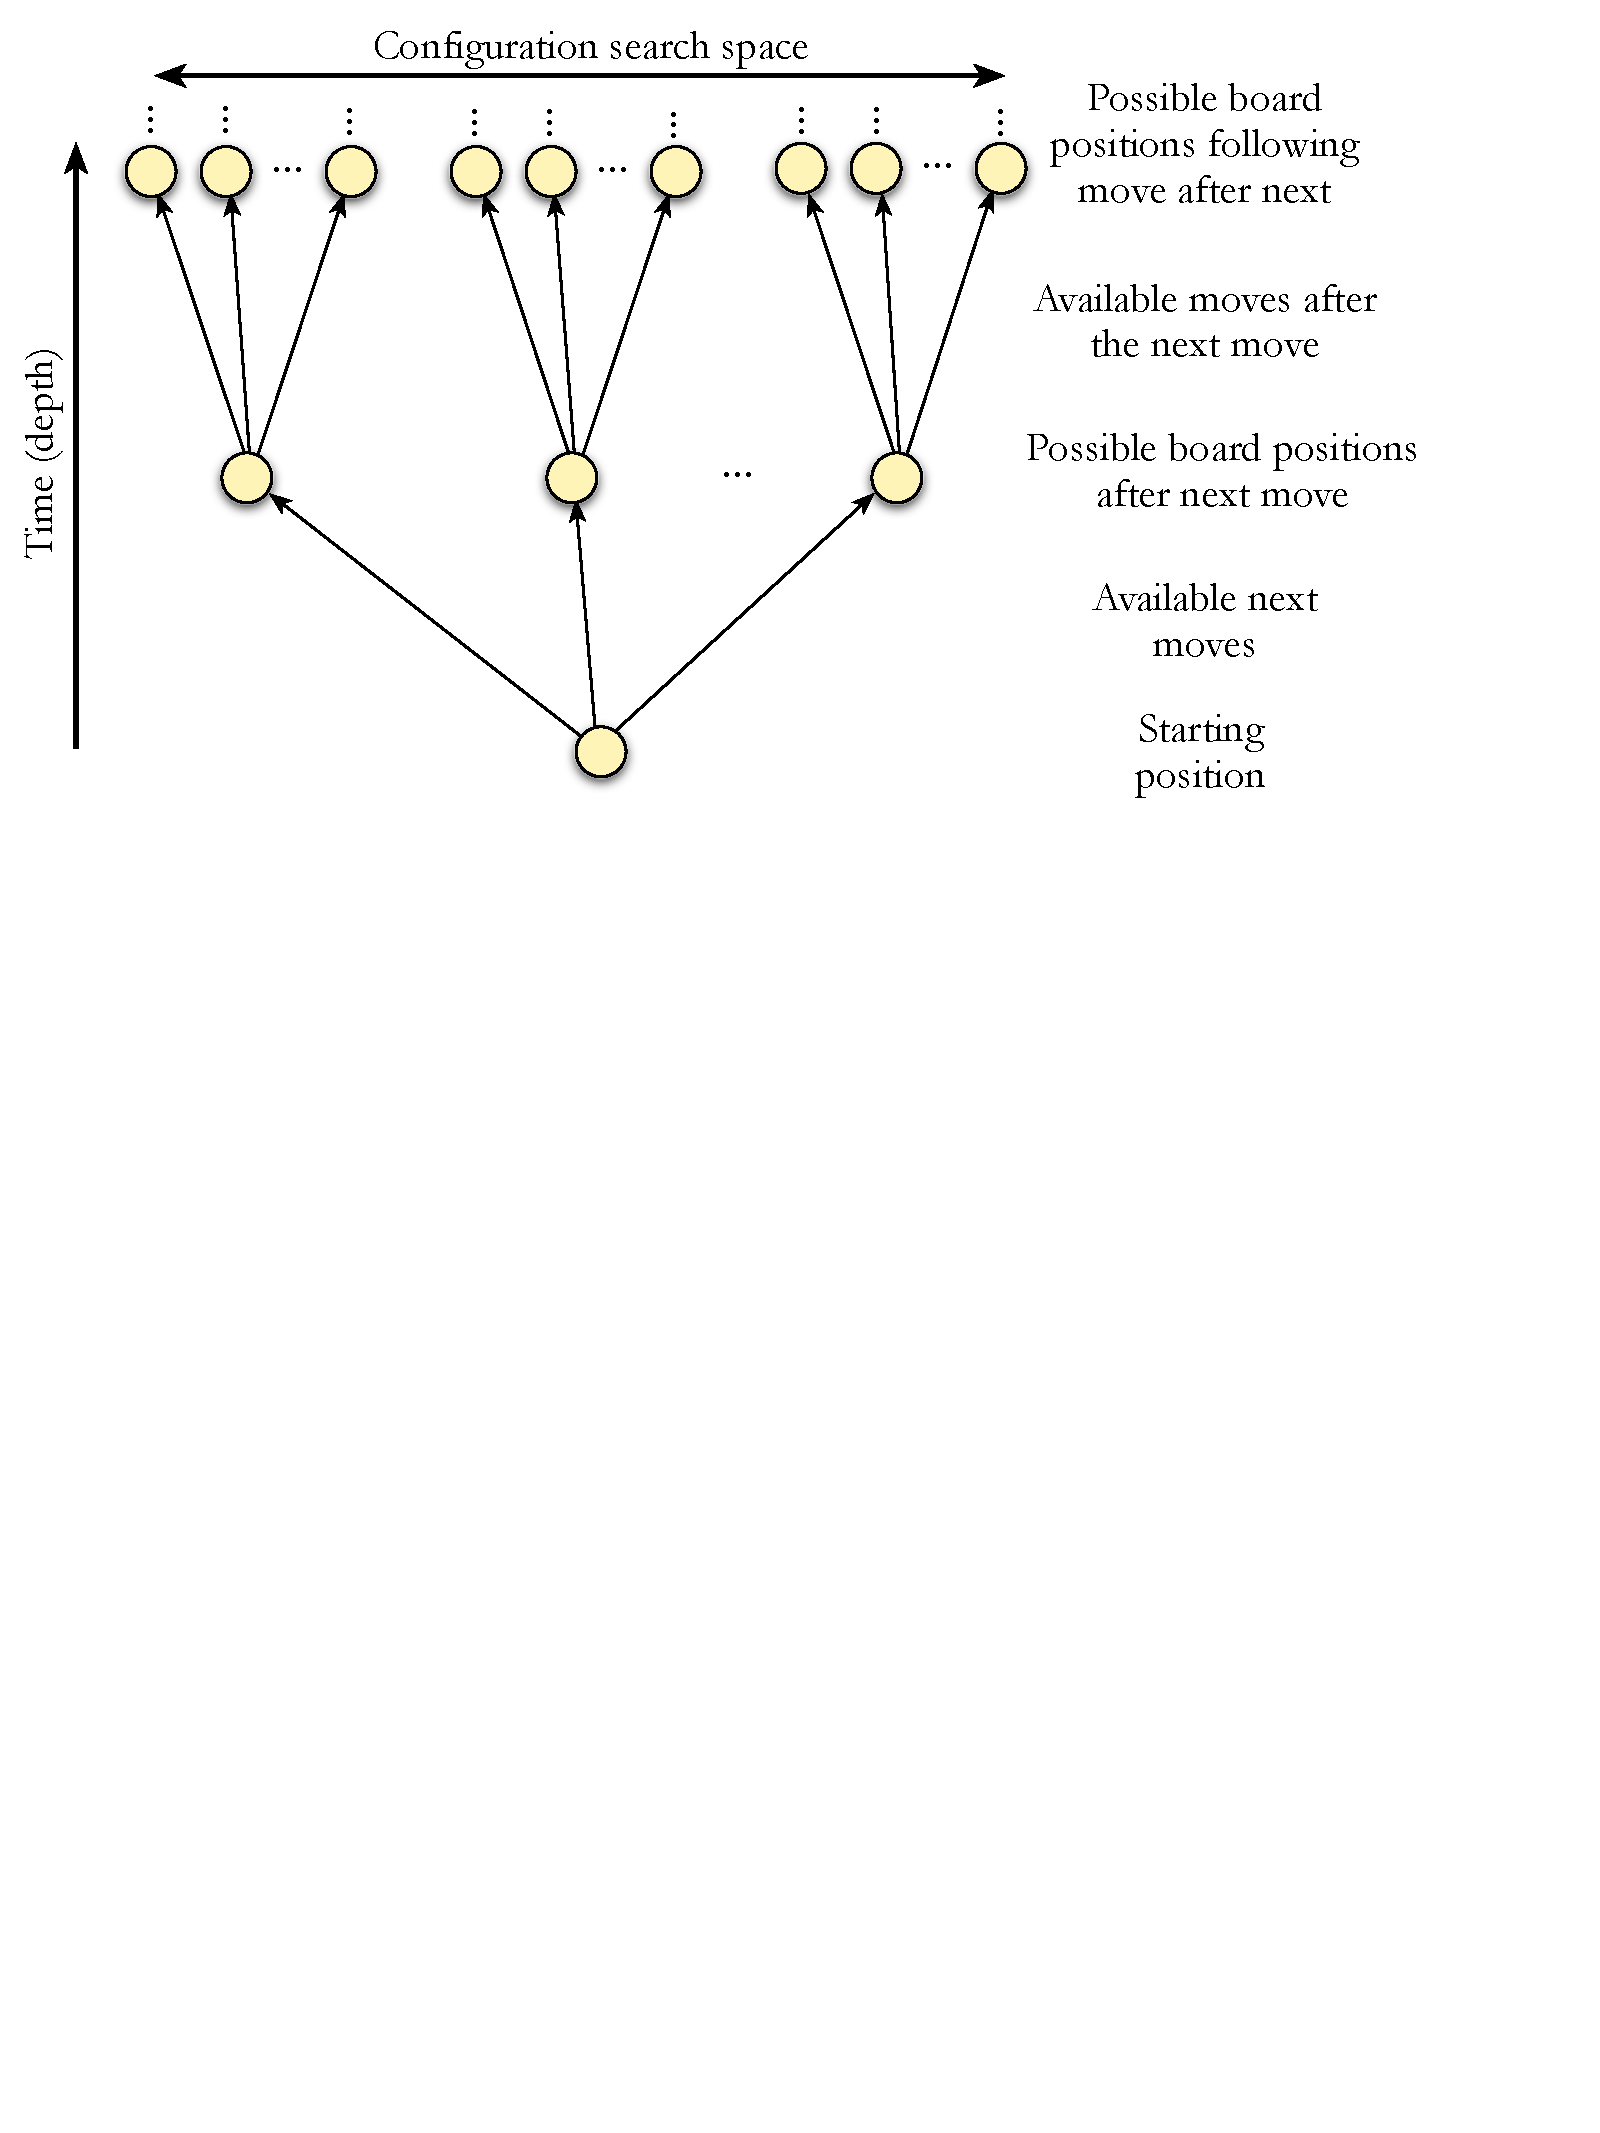
\includegraphics[width=0.47\textwidth]{search_tree}
	\caption{A search tree\index{Search tree} is an outwardly-directed tree graph in which each vertex represents a state of the system (i.e `board position' in chess\index{Chess}). Edges represent actions (or `moves') available from the position from which the edge emanates. The root node represents the current position, and the depth of a vertex (i.e it's distance from the root node) represents its future time. A path through the tree therefore represents a sequence of moves up to some point in future time. If the tree had maximum depth, a route (from root to leaf) would represent an entire single game, and the complete set of routes would represent all possible ways in which the game can be played. A complete analysis of a complete search tree with maximum depth would therefore allow us to exhaustively analyse all possible ways in which a game could be played to completion, enabling optimal gameplay. However, since the number of vertices/edges in a tree graph grows exponentially with depth, the configuration search space in a game grows exponentially with how may moves into the future we wish to explore, thereby strongly limiting tree depth in practical implementations.}\label{fig:search_tree}
\end{figure}

This approach lends itself ideally to approximation via Grover. We take the same classical board-position-scoring algorithm, and implement it as an oracle. Grover is then able to search through a quadratically larger search tree, querying the oracle for scores above threshold.

Indeed this intuitive example is a very powerful one -- since all \textbf{EXP}-complete problems are by definition equivalent, and \textbf{EXP} contains many other lesser (but hard) classes, the approximate optimisation technique immediately captures a vast array of interesting problems.

\subsection{How beneficial is quantum-enhanced optimisation?}

The utilisation of Grover's\index{Grover's algorithm} algorithm as the basis for improving optimisation problems may seem a little depressing, given that quantum search algorithms only confer a modest quadratic enhancement. By comparison, so many other quantum algorithms offer exponential speedup! How significant is such a quadratic enhancement actually?

In the context of a search tree\index{Search tree}, the size of the search space\index{Search space} (i.e number of leaves on the tree) is \mbox{$s=b^d$},
where $b$ is the tree's branching parameter (assumed uniform here for simplicity) and $d$ is tree depth. A quadratic enhancement in the searchable search space to \mbox{$s'=s^2$} effectively doubles the search tree depth that can be accommodated by a given number of oracle calls to \mbox{$d'=2d$}.

Needless to say, doubling one's foresight in planning for the future is highly advantageous and could lead to huge improvements in competitive advantage and efficiency in resource allocation. Doubling the number of moves a competitive chess\index{Chess} player could look ahead would result in their complete and utter dominance of the game!

Despite all this optimism, there remains one major concern, one shared by any quantum algorithm offering only polynomial enhancement. In any real-world quantum computer fault-tolerance\index{Fault-tolerance} is necessarily required to enable the algorithm to be executed faithfully in the inevitable presence of noise. However, fault-tolerant codes necessarily induce a time and space overhead (i.e in terms of the number of physical qubits, and algorithmic runtime). If this overhead is too large it could well overpower the   enhancement offered by the underlying algorithm. For this reason, real-world implementations of these types of algorithms will require very careful consideration of the construction of their associated error correction circuitry, such that there is still some net tangible algorithmic gain at the end. The quadratic enhancement in algorithmic runtime is actually a bound based on the ideal-case where there are no errors. In a fault-tolerant construction the actual achievable enhancement will necessarily be less than this. Specifically, for a given runtime, if the enhancement in the searchable search space is a polynomial of order $p$, this equates to an effective increase in search tree depth by a factor of $p$.

\subsection{Implications for the future}

While the dream-goals of perfectly optimised resource allocation and perfect economic efficiency are fantasy, we should not underestimate the impact that even modest enhancements in the efficiency of large-scale economic systems could have. While quantum computers will never perfectly solve humanity's immense resource allocation problems, even the more modest improvements they offer could be of immense value to the world economy, with enormous implications monetarily, socially, and environmentally. Indeed, optimisation problems are so ubiquitous that pursuing quantum-enhanced optimisation will be of central importance in the quantum era.